\chapter{\signpost: Internet-scale secure and scalable connectivity}
\label{sec:signpost}
\ifpdf
    \graphicspath{{Chapter3/Chapter3Figs/PNG/}{Chapter3/Chapter3Figs/PDF/}{Chapter3/Chapter3Figs/}}
\else
    \graphicspath{{Chapter3/Chapter3Figs/EPS/}{Chapter3/Chapter3Figs/}}
\fi

In this chapter we explore applications of the SDN technology in connectivity
scalability.  The work is motivated by a common network use-case, seamless
information and resources sharing between the devices of a user.  We call this
functionality Personal Cloud.  Currently, Personal Clouds functionality employs
Cloud services as information caches which bridge the required inter-device
communication. This architecture is a consequence of the connectivity
scalability limitations experienced by network applications, as discussed in
Section~\ref{sec:intro:motivations}. Nonetheless, as users offload personal
information to third party services, they become subject to privacy threats and
performance degradation.

We argue that end-devices require an adaptable network control architecture, in
order to overcome the network connectivity limitations and regain control of
their data by establishing user-managed Personal Cloud.  We propose \signpost,
an evolved network control plane for end-devices, delivering continuous and
secure connectivity between the devices of a user. \signpost integrates existing
network testing approaches to detect network environment conditions and
configures existing software packages to establish end-to-end connectivity
between devices. 

In order to understand the feasibility and performance of the proposed
architecture, we present a strawman implementation of the core control logic of
the proposed architecture and its integration with a number of network
connection and notification services.  Currently, \signpost supports SSH,
OpenVPN, TOR, NAT-punch and Privoxy connection mechanisms, while it can also
propagate Multicast-DNS notifications across devices.

For the rest of this chapter, we present a preliminary categorisation of
Personal Cloud platforms and,
motivated by some key observation, we define the key design requirements for our
platform~(Section~\ref{sec:signpost-introduction}). Furthermore, we present the
\signpost design~(Section~\ref{sec:sp-signpost}) and  
architecture~(Section~\ref{sec:signpost-architecture}), followed by an elaborate
description of a strawman implementation of the system and an evaluation of its
functionality~(Section~\ref{sec:signpost-evaluation}).  Finally, we conclude our
observations~(Section~\ref{sec:signpost-conclusion}).

% The architecture provides two points of integration with legacy applications. 
% From the user perspective, the system integrates functionality on the
% network layer of the OS, thus providing backward compatibility with existing
% applications on the forwarding path. Additionally, the design provides a 
% user-friendly naming abstraction to devices, over the DNS protocol. DNS
% lookups for device names establish an API for applications to request from 
% the system the establishment of a path between 2 devices; a mechanism which we
% call {\it ``Effectful Naming''}.

% The propose architecture utilizes \of-enabled bridge and a
% local controller on each device. Each controller by default forwards packets as
% normal on the local network. The forwarding logic, though,  is augmenting
% through a distributed coordination protocol which permits nodes to negotiate
% possible connection opportunities and establish ad-hoc tunnels, enabling as a
% result an Internet-wide distributed control mechanism. 
% At the core of
% our design, we  the naming service host abstraction. Each device
% acquires a global domain name, while each name resolution triggers a connection
% engine, that tries to find the best possible bidirectional channel between the
% two nodes. The naming service uses the established
% DNSSEC extension, providing a fully authenticated and secure control
% mechanism among \signpost and applications. Further, the distributed nature
% of the naming hierarchy in the Internet permits seamless control distribution.

\section{Personal Clouds}\label{sec:signpost-introduction}

% Numerous applications and protocols have been developed to fulfil Personal Cloud
% functionalities, such as remote desktop access, file sharing, remote login,
% remote printing etc.   Such applications extend the computer abstraction with
% mechanisms providing information and resource sharing between devices.  

In the recent years, the global increase in the adoption of personal computers
has mirrored a large part of our life in the digital domain. For example, human
labour is commonly stored in digital PDF and word processing files, while
digital photo collections express a part of our social interactions.  As a
result, our physical presence has an increasing digital counterpart. A user
interacts primarily with his digital presence through his computing
devices. Although, the recent increase in the number of computing devices per-user
introduces new challenges in the management of our digital presence.
Complimentary to their personal computer, users on average currently own and use
a tablet, a smartphone and a variable number of purpose-build computing units
for home entertainment and gaming.  Each user device fulfils specific
roles in managing the user digital resources, thus requiring access only to a subset of the user digital
presence, but these roles are fluid and intercept.  For example, a smartphone is
primarily a communication device, but end-users may use it as a media player. In
the latter case, the smartphone and the home entertainment system provide
similar functionality to the user and require access to the same subset of his
digital presence. This transition from the single PC paradigm to the
multi-device paradigm and the concurrent digital footprint augmentation create a
user requirement for new services providing global and homogeneous access and
control of personal digital information and resources. We call this abstraction
the user \emph{Personal Cloud}. 

In the rest of this Section, we present existing mechanisms providing Personal
Cloud functionality~(Subsection~\ref{sec:sp-approaches}) and discuss their
functional limitations in order to define the design goals for our \signpost
system~(Subsection~\ref{sec:sp-challenges}). 
% and introduce readers to the
% \signpost framework~(Subsection~\ref{sec:sp-signpost}).

\subsection{Approaches} \label{sec:sp-approaches}

% Although reachability is reduced, Internet remains a highly performant and
% connected system; it interconnects billion of users and transports Terrabytes of
% information daily. This is achieved due to the predominant operational model of
% Internet services. Hosts in the common case connect to a small subset of the
% Internet space that provides access to popular information.  This model, which
% is called {\it Client-Server model}, is a natural result of the power-law
% chatacteristics of various social and engineering mechanisms. Internet network
% graph is a power law graph, due to its scalable hierarchical structure, while
% information popularity exhibits strong power law characteristics. 

Currently, partial Personal Cloud functionality is readily available in a number
of applications. Such applications provide a wide range of abstractions and each
has different network resource and connectivity requirements. We group these
approach in two distinct categories, based on the service architecture. 

\paragraph*{Decentralised Personal Cloud}

The requirement to share information and computing resources has been a core
application for computer networks since their introduction. Currently the
average user has access to a large number of free software packages and
protocols that provide Personal Cloud functionalities, such as remote desktop
access (e.g.~Remote Frame Buffer protocol~\cite{RFC6143}), file sharing
(e.g.~NFS~\cite{RFC3530}, SAMBA file service~\cite{samba}), remote login
(e.g.~SSH~\cite{RFC4253}), remote printing (e.g.~IPP~\cite{RFC2911}) etc.\
between devices. Such applications follow the client-server connection paradigm
and extend the computer abstraction to accommodate inter-device connectivity and
resource accessibility. A user can setup and manage the equivalent services on
his personal devices and enhance his user experience with Personal Cloud
functionality.  In addition, the network community has developed mechanisms to
ease the configuration of such services.  Multicast-DNS, UPnP and ZeroConf
protocols allow a user to seamlessly browse and access available services upon
connection to a network. 

Decentralised Personal Cloud applications enable users to fully control their
digital footprint and provide strong privacy guarantees. Data are stored on
users devices and the user has full control on the propagation of his
information.  Nonetheless, deploying such service in the Internet raises
significant scalability issues. We focus on three significant problems in
Internet-scale deployments. 
% : {\it
%  Connectivity}, {\it Authentication} \/and {\it Usability}. 

\begin{itemize}
  \item {\it Connectivity}\/: Current Internet architecture cannot guarantee
        globally accessible services for all hosts, as we have discussed in
        Section~\ref{sec:intro:motivations}, and as a consequence the
        effectiveness of the Client-server model of decentralised Personal Cloud
        applications is limited.  End-users commonly connect to the Internet
        through edge networks optimised for outgoing connectivity and
        transparent middleboxes commonly violate the Rubstness principle of the
        Internet. For example, NATed networks, that scale addressing on the
        edges of the network, limit incoming Internet connectivity for a
        significant number of devices and require manual configuration to expose
        services. Similarly, mobile and enterprise networks employ firewalls to
        restrict publicly accessible services on connected hosts for security
        reasons.
  \item {\it Authentication}\/: Distributed Personal Cloud applications employ
        an inflexible authentication mechanism, based on pre-shared passwords
        and public keys. Access to a decentralised service requires a secure
        channel to negotiate  a-priori the security credentials for a user,
        while access control is integrated in the service configuration. 
  \item {\it Usability}\/: Decentralised Personal Cloud applications introduce
        configuration requirements which dim them inappropriate for
        inexperienced users. As we have already discussed in
        Section~\ref{s:home_social}, the average end-user is highly unlike to
        engage in systematic service configuration of decentralised services,
        since the configuration tasks are long and complex. Decentralised
        Personal Cloud services contain network functionality assumptions and
        users may need additional software layers, like tunneling software, to
        achieve functionality.  In addition, as network policies exhibit
        variability, a user must resolve to ``trial and error'' approaches to
        evaluate which end-host configuration is effective in a specific
        environment. \\ 
        As an example, we describe the steps required to access files from a
        remote device using the SSH service. Before the user is able to
        connect to a computer over SSH, he has to configure the service on his
        server machine, both in terms of access control and service
        functionality, as well as, any firewall and NATbox  services deployed in
        the local network. Additionally, an IP resolution service is required if
        the public IP of the server is dynamic, 
        e.g.~DynDNS~\footnote{\url{http://dyn.com/dns/}}\@.  SSH connectivity is
        subject to the ability of the user in the remote network to use the SSH
        protocol over the preconfigured port.  In case this is not possible, the
        user has to try a different connection establishing mechanism.
\end{itemize}

\paragraph*{Centralised Personal Cloud}

A popular alternative to decentralised Personal Cloud services uses cloud-based
services to bridge information flows between devices.  In this group we consider
applications like the Google service suite, Dropbox file sharing service,
LogMeIn Remote Desktop service and other alike services.  These applications
provide a simple, intuitive and ubiquitous mechanism to store and retrieve data
between the devices of the users or a specific subset of users from the service
extensive user-base, providing the ability to extend the sharing capabilities
with a user social circle. For example, Google Docs allow users to store online
documents and process them in parallel with a defined set of online friend.
Although this approach provides all required functionality, some of design
points of the architecture are ambivalent and demotivate user engagement. 

\begin{itemize}
  \item{\it Identity}\/: Cloud applications provide an effective control
       framework to disseminate information between devices and users.  Users
       define information access policies based on online identities and the
       service ensures secure delivery.  Nonetheless, as a service becomes
       popular and its functionality is integrated with third-party
       applications, the service provider gains the ability to identify users to
       third parties or monitor registered users.  In~\cite{Krishnamurthy2009}
       the authors report a case of identity exposure by Online Social Networks
       to advertising services, in an effort to detect and characterize user
       interests.  Facebook has openly verified the existence of such
       services~\cite{beacon-facebook}. 

\item {\it Performance}\/: The elasticity of cloud computing infrastructures
      enables centralise Personal Cloud services to provide scalable
      performance, irrespective of data volumes and service popularity.
      Nonetheless, the service architecture underutilizes the wealth of
      computational and network resources available in end-user devices.  Two
      devices connected to the same subnet will experience bloated RTT values
      when they communicate through a cloud service, while the cost and
      performance of cloud storage resources is orders of magnitude higher in
      comparison to the cost of local storage.  In~\cite{Wittie2010}, authors
      report a significant impact on the 95th quantile network performance of
      cloud services, due to latency and packet losses incurred by the Internet,
      while in~\cite{Dean13} the authors present a wide range of parameters,
      spanning from the CPU scheduler to hardware design, which influence
      user-perceived performance.
%       \todo{Add dropbox measurement study}

\item {\it cost}\/: A large number of centralised Personal Cloud services, like
      iCloud and Dropbox, allow limited service usage free of charge, to
      increase popularity and develop new monetisation mechanisms.  Nonetheless,
      the user service level agreements~(SLA) for the class of free users
      provides minimum guarantees. For example, if a part of the service is
      compromised and sensitive information are leaked, the SLAs minimize the
      obligations of the provider towards affected users~\cite{cnet-dropbox}.
      Such costs are not directly observed by an end-user, but they can impact
      significantly his social and work experience. 

\item {\it Availability}\/: Cloud services run on well connected
      infrastructures, monitored by highly-skilled engineers to ensure
      performance, functionality and security. Service functionality requires
      only outgoing Internet connectivity.  However, the centralised
      architecture of such services introduces a single point of failure in
      inter-device communication. For example, two devices, belonging to
      different users and connected to the same local network, cannot exchange a
      file over Dropbox, if the firewall policy forbids connectivity with the
      Dropbox servers~\footnote{Dropbox provides local network synchronization
        functionality between devices, which though is used only for performance
        reasons and require service
        connectivity~\url{https://www.dropbox.com/help/137/en}}. 

% \item {\emph Generality}\/: Cloud applications develop distributed services
%       optimized for specific functionality. Google Drive provides online
%       document storage, Youtube provides online video hosting and Facebook
%       provides Online Social Network Services. Users are limited on their ability
%       to share information or resources by the offered capabilities of the
%       service provider and there isn't a sole service provider that can
%       support functionality for the complete ensemble of Personal Cloud services. 
\end{itemize}

\subsection{Design Goals} \label{sec:sp-challenges}

In the previous section, we present the capabilities and limitations of existing
Personal Cloud applications. Decentralized Personal Cloud applications luck
user-friendliness and their functionality is subject to the network
policy. On the other hand, centralised Personal Cloud architecture introduces
privacy vulnerabilities~\cite{facebook-nsa} and performance bottleneck.  

We believe that an efficient and secure Personal Cloud framework should employ a
hybrid approach to scale the problems of connectivity, security and usability.
User information should be stored on user-managed devices and the system must
provide user-controlled privacy.  The wealth of available decentralized Personal
Cloud applications  provides a sufficient set of applications to support the
required functionality.  Nonetheless, Personal Cloud functionality cannot ensure
Internet-wide inter-device connectivity, without the usage of cloud services.
Cloud support is required in order to establish  a control channel between the
instances of the system. Additionally, data plane end-to-end connectivity can be
achieved over the Internet, without cloud mediation, by appropriate testing and
configuration of existing connection establishing software.  We set the
following high-level goals for our system architecture:

% The data plane of the system should use multiple and
% different connection mechanisms, in order to optimize the performance and
% security of the resulting end-to-end paths. Each device control plane should be
% able to detect network restrictions and use existing mechanisms to bypass them,
% while off-line functionality should also be available when possible. 

\begin{itemize}
  \item {\it Connectivity}\/: A personal cloud architecture must provide
        connectivity, and thus functionality, in all network environments.
        The system should be able to recover functionality when exogenous
        factors disrupt connectivity.     
%     The framework should provide a control plane
%         optimized to enable inter-device communication.  The design of the
%         control should decouple inter-device communications from the network
%         state of the device, in order to dynamically optimise the performance of
%         the end-to-end path. In addition, the resulting connection abstraction
%         should be able to recover from network disconnections.

  \item {\it Control}\/: A Personal Cloud system should expose a user-friendly
        access control abstraction.  Access policies should operate on the level
        of devices or users and rely on strong authentication and encryption
        mechanisms. Additionally, the control should be sufficiently dynamic to
        respond to security changes, e.g.~propagate trust revocation for a
        compromised device. In addition, the control abstraction should
        incorporate diverse security aspects and allow the user to control the
        trade-offs between performance and security.
   
  \item {\it Backward Compatibility}\/: The framework should provide support to
        existing decentralised applications without any modification of their
        functionality.

  \item {\it Usability}\/: The system should expose a simple control abstraction
        to end-users in order to orchestrate the connection establishment
        process. All low-level networks interactions should be managed by the
        system and remain hidden by the end-user. Ultimately, the
        abstraction of the system should be compatible with the existing
        functionality of decentralised Personal Cloud. 
    
%    Individuals need to have a memorable way to refer to devices. 
%    The naming service should dynamically adjust to the state of devices, provide global
%    coverage, be scalable and provide some partial mechanisms to obfuscate users
%    connection interest toward other entities. Additionally, the naming service
%    should provide a mechanism to detect unauthorized users as well as protocol
%    modifications.

 \end{itemize}

% Personal cloud computing requirements currently experience a mismatch with the
% functional properties of the Internet.  Personal devices usually connect to
% networks optimised for outgoing connectivity and various components of the
% Internet are not designed to accommodate well-connected services for every host.
% NATed networks, that scale connectivity on the edges of the network, require
% manual configuration in order to host Internet-reachable services, while a
% number of edge networks, namely mobile and enterprise networks, restrict
% publicly accessible services on connected hosts for security reasons. In order
% to overcome these restrictions a number of approach has been proposed by the
% research community, as well as the industry.  We group these solutions in the
% following two categories:

% Internet is an excellent example of a dynamic system managing to address
% effectively evolution.  In the early days of the system, in
% order to extend user adoption, its  steering committee set simplicity and
% openness as two fundamental design goals. Due to these design choices, Internet
% protocols gained rapidly support by a wide range of OSes, while the set of
% connected entities augmented exponentially.  Nonetheless, during that period, the
% Internet remained a large wide area network, interconnecting research
% institutes, and the predominant applications provided constraint relaxed
% asynchronous communication. Through the years though, and as Internet users
% increased, new applications emerged and highlighted a number of
% security and performance limitation in the initial design of the system.
% 
% In order to address these limitations in a backward compatible manner, a number
% of network hacks were introduced in the Internet design. One of the most popular
% hack is the deployment of middleboxes~\cite{RFC3234}.  Middleboxes violate in a
% number of ways design principles of the Internet, in order to provide an
% effective framework to ``inject`` functionality that addresses design
% limitation. For example, \emph{NATboxes} handle the IPv4 address space shortage,
% \emph{WAN optimizers} improve utilization of under-provisioned links, while
% \emph{firewalls} secure critical networks.  Unfortunately, Middlebox deployment
% redefines to a great extend the Internet abstraction. A number of papers have
% described their impact: in~\cite{Honda:2011ci} authors pinpoint middlebox
% functionality as a core cause in the ossification of the transport layer, while
% in~\cite{Kreibich10} authors describe a wide range of protocol functionality
% that has become suppressed due to middlebox functionality. 
% % Mainly, due to middlebox functionality, the
% % initial design properties of the system in terms of simplicity and openness have
% % been lost for a large subset of the Internet.  
% 
% \todo{ describe some efforts to overcome middleboxes.}
% \todo{IPv6 can do some of that,but not everything }
% An important impact of middlebox deployment is the reduced connectivity
% introduced in the Internet. Home networks host a number of hidden devices which
% remain inaccessible from the Internet due to NATbox functionality, while strict
% firewall policies in enterprise networks reduce protocol functionality.
% Personal Cloud deployment across the Internet is increasingly restricted, as
% devices are not able to interconnect directly.


\section{Finding your way with \signpost}\label{sec:sp-signpost}

\signpost is a Personal Cloud-enabling framework with user-controlled security.
The system provides an Internet-wide overlay network abstraction between the
devices of a user to enable primarily decentralised Personal Cloud
functionality.  \signpost uses a cloud-based inter-device control channel to
coordinate end-to-end network path establishment between devices, using existing
connection establishing software and protocol.  In order to ensure functionality
under any circumstance, the \signpost control channel is integrated with the
Internet naming service, a high availability and resilient service. 

\signpost design defines a generic testing and configuration model which
automates the process of connection establishment for a wide range of relevant
software.  The system design provides seamless integration with existing
applications. The applications can use \signpost paths by routing traffic to a
\signpost specific address, while the control API for inter-device connection
establishment is integrated with the \textit{gethostbyname()} OS method.  Each
device is exposed to the users as a domain name and a name lookup for a device
triggers the \signpost connection establishment mechanism. Finally, \signpost
exposes a security control interface through which users can demand specific
security properties for their inter-device paths. As a consequence, the user
controls the security properties of inter-device information dissemination,
while avoiding privacy-sensitive cloud service data offloading. 

\begin{figure}[ht]
  \begin{center}
	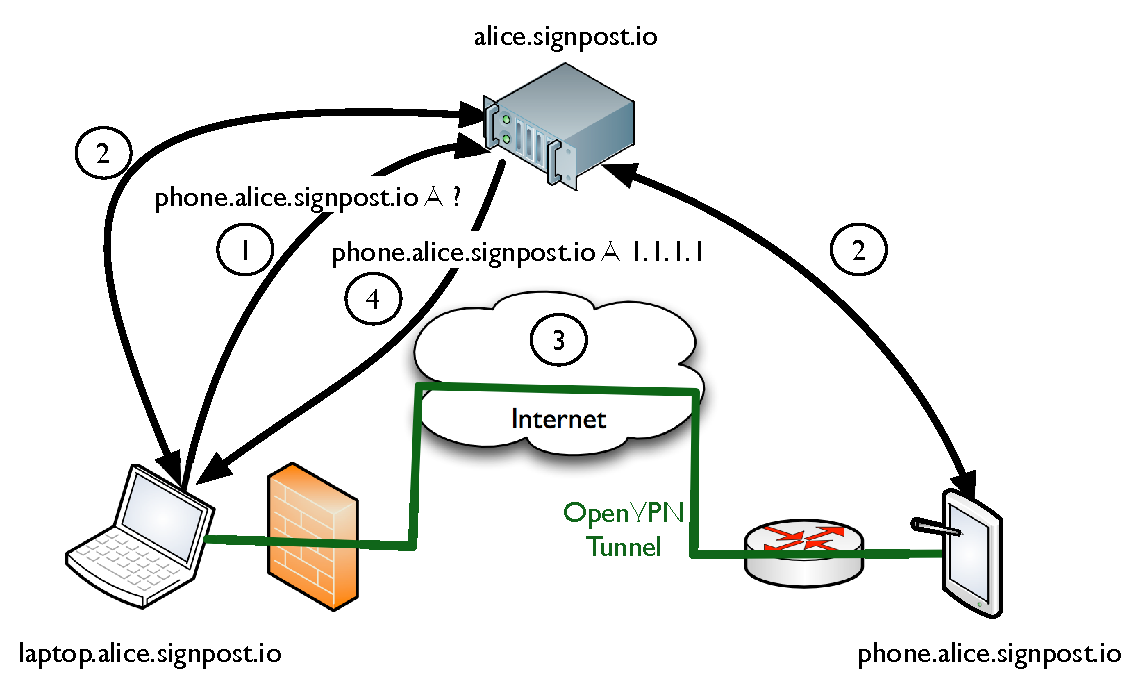
\includegraphics[width=0.6\textwidth]{Chapter3/Chapter3Figs/sp-illustration}
  \end{center}
  \caption{A simple example of the \signpost abstraction when the user Alice
    interconnects a smarthphone with the home computer over the Internet.}
  \label{fig:signpost-user-abstraction}
\end{figure}

In order to introduce the reader to the \signpost abstraction, we depict in
Figure~\ref{fig:signpost-user-abstraction} a simple use case example.
In this scenario user Bob, while at work using his smartphone,
wishes to access some files on his laptop, situated behind his NATing home
router. In order to express his interest to connect to his laptop, Bob performs
a name lookup for the domain name \fqsn{laptop.bob} to his local \signpost
resolver~(step~\ding{192}).  The name request propagates through the public DNS
infrastructure to his \signpost cloud service, which we call the {\it \signpost
  controller}. A verified name request to the \signpost controller initiate the
connection establishment logic of the system, which triggers the two devices to
try multiple connection establishment mechanisms and setup an
end-to-end path~(step~\ding{193}). Once an initial path becomes
available~(step~\ding{194}), the controller replies to the initial name request
with a local \signpost-specific IP address. Traffic to this address is routed by
the device network stack to the established inter-device network
path~(step~\ding{195}).  In parallel, \signpost continues to evaluate different
connection establishing mechanism, aiming to optimize the utilized path, and
monitors path availability, in order to recover connectivity in case of
a disconnection. 

% Our work builds on the observations on the shortcoming of current approaches to
% interconnect devices, and tries to bridge the two domains, providing the
% appropriate control mechanisms to end-users. On one hand, we want to
% model a generic framework that will allow end-host to automatically test the
% network environment, discover the optimum mechanism to interconnect two
% devices and distributely negotiate the connection parameters with other devices,
% without any user interaction. On the other hand, we want to provide to the users
% a mechanism that will allow them to control to a great extend the security and
% privacy of their information. 

% §develop and deploy various protocol modifications that tried to bypass these
% design flaws.  Unfortunately, such systems tend to introduce stricter
% assumptions on how the network should function, and reduce to a great extend the
% openess of the Internet.There are primarily two major classes of engineering
% modifications that reduce network connectivity: performance enhancing
% middleboxes and edge-network security policy reinforcement.  
% Performance
% enhancing middleboxes are network forwarding devices, installed in the network,
% that aggregate information from multiple layers of the TCP/IP stack and modify
% packet content or forwarding logic. 
% This restriction in openess of some parts of
% the Internet is a vital reason for the inability of the network community to
% establish Private Clouds across the Internet.  


% \section{\signpost Design Goals} \label{sec:signpost-goals}

\section{\signpost Architecture}\label{sec:signpost-architecture}

\begin{figure}
  \begin{center}
	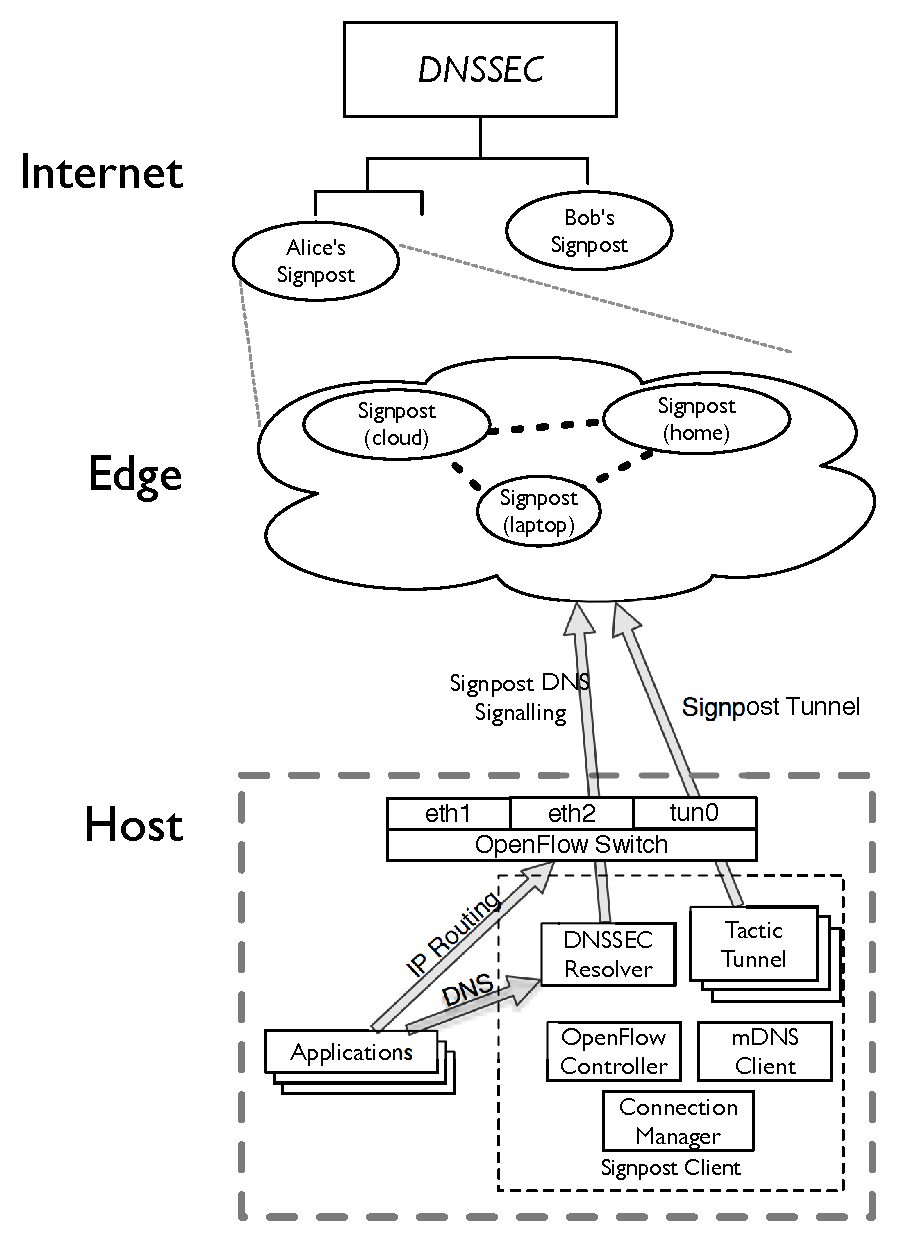
\includegraphics[width=0.9\textwidth]{signpost-arch}
  \end{center}
  \caption{\signpost architecture}
  \label{fig:signpost-arch}
\end{figure}

% \signpost is an Internet-wide secure inter-device communication system. The
% system reuses existing Internet protocols and connectivity mechanisms and
% provides an overlay local network. 

In Figure~\ref{fig:signpost-arch} we present
a diagram of the \signpost architecture over different viewpoints. 
%%
In the lower section of the figure, we present the design of the \signpost
software and its integration with existing applications.  \signpost logic is
contained in a single executable, and requires from the guest OS to expose an
\of switch interface and to redirect DNS queries to the embedded DNS resolver.
The software consists of three subsystems: The {\it Connection
  Engine}~(Subsection~\ref{signpost-engine}), responsible to set up and manage
{\it Network Tactics}~(Section~\ref{signpost-tactic} in order to establish
end-to-end paths, the local DNS resolver and the \of-based {\it \signpost
  router}~(Section~\ref{signpost-forwarding}) which enhances the normal OS
routing functionality with \signpost network control logic.  
%%
In the middle layer of Figure~\ref{fig:signpost-arch}, we present the control
plane interconnection between \signpost devices. The system setups an
Internet-wide inter-device control channel to enable capability and parameter
negotiation between devices. The architecture requires a special \signpost node,
which we call \emph{\signpost Controller}, to run on a well-connected host and
bridge the device control channel across the Internet and orchestrate
connectivity establishment. \signpost, in addition, provides off-line
authenticated connectivity between devices connected to the same network, by
exploiting the service discovery functionality of the Bonjour protocol. 
%%
In the upper layer of Figure~\ref{fig:signpost-arch}, we present the naming
organisation of the \signpost architecture. The system reuses the naming
abstraction of the DNS service. Each device has a global domain name, while the
domain hierarchy and name aliasing expresses the control relationship between
devices and users.  We extend the normal name resolution functionality of the
DNS protocol and introduce the  {\it Effectful name resolution} operation for
\signpost-enabled domains; a name resolution expresses the interest of a user to
establish an end-to-end path~(Subsection~\ref{signpost-naming}). For the rest of
the section we present in detail the architecture of the \signpost system. 

\subsection{Network Tactic} \label{signpost-tactic}

\begin{table*}
\centering \footnotesize
\begin{tabular}{|l|c|c|c|c|c|c|p{1.5cm}| }
  \hline
  Tactic name & Purpose & Layer & Transport & Auth. & Encrypted & Anon. & \signpost
Support\\
 %% & Comment & Source \\
\hline
Avahi       & Discover         & 7      & UDP         & No     & No     & No & Yes\\
 %% & Linux-based, bonjour-compatible system for local network resource discovery
 %% & \url{avahi.org/} \\
Samba       & Discover         & 7      & UDP         & No     & No     & No & No \\
 %% & Windows local network resource discovery protocol, implemented in WINS & \\
Bonjour     & Discover         & 7      & UDP         & No     & No     & No & Yes\\
 %% & Used for local network resource discovery
 %% & \url{developer.apple.com/opensource/} \\
Universal PnP & Discover         & 7      & UDP         & No     & No     & No & Yes\\
dns2tcp     & Tunnel             & 7      & UDP         & No     & No     & No & No \\
 %% & IP over DNS & \url{www.hsc.fr/ressources/outils/dns2tcp/index.html.en} \\
DNScat      & Tunnel            & 7      & UDP         & Yes    & No     & No & No \\
 %% & VPN with PPP & \url{tadek.pietraszek.org/projects/DNScat/} \\
HTTP-Tunnel & Tunnel            & 7      & TCP         & No     & No     & No & No \\
 %% & uses HTTP & \url{www.nocrew.org/software/httptunnel.html} \\
iodine      & Tunnel            & 7      & UDP         & Yes    & No     & No & Yes\\
 %% & IP over DNS & \url{code.kryo.se/iodine/} \\
NSTX        & Tunnel            & 7      & UDP         & No?    & No     & No & No\\
 %% & IP over DNS. Deprecated. Recommends iodine 
 %% & \url{thomer.com/howtos/nstx.html} \\
% IMAP        & Data transfer     & 7      & TCP         & Can be & Can be & No \\
 %% & & \\
Proxytunnel & Tunnel            & 7      & TCP         & Can be & Can be & No & No\\
 %% & can use both HTTP and HTTPS & \url{proxytunnel.sourceforge.net/} \\
ptunnel     & Tunnel            & 4      & ICMP        & Yes    & No     & No & No\\
tuns        & Tunnel            & 7      & UDP         & &        No     & No & No\\
 %% & IP over DNS. Doesn't split IP packets, but sets size so small that OS does
 %%   fragmentation. Neat. Only uses CNAME for maximum compatibility with
 %%   infrastructure. Poor performance :( 
 %% & \url{www.loria.fr/~lnussbau/tuns.html} \\ 
SSH         & Tunnel/Encrypt & 7      & TCP         & Yes    & Yes    & No & Yes\\
IPSec       & Tunnel/Encrypt & 3 (4*) & IP          & Yes    & Yes    & No & No\\
 %% & In layer 4 when traversing NATS (over UDP or TCP) & \\
OpenVPN     & Tunnel/Encrypt & 7      & UDP/TCP     & Yes    & Yes    & No & Yes\\
 %% & & \url{openvpn.net/} \\
libjingle   & Nat punch         & 7      & UDP/TCP     & Yes    & ?      & No & No\\
 %% & For punching holes. Negotiation over XMPP
 %% & \url{code.google.com/apis/talk/libjingle/index.html} \\
privoxy     & Anonymize         & 7      & TCP         & ?      & ?      & Yes & Yes\\
tor         & Anonymize         & 7      & TCP         & No     & Yes    & Yes & Yes\\
 %% & & \url{www.privoxy.org} \\
% SMTP        & Data transfer     & 7      & TCP         & Can be & Can be & No \\
stunnel     & Encrypt        & 7      & TCP         & Yes    & Yes    & No & No\\
TCPCrypt    & Encrypt        & 4      & TCP         & No     & Yes    & No & No\\
\hline
\end{tabular}
\caption{\label{tbl:signpost-tunnels}Tactics table.}
\end{table*}

In order to provide end-to-end connectivity, \signpost reuses the wide range of
free and open source connection establishing mechanisms developed by the
research community. In Table~\ref{tbl:signpost-tunnels}, we present a small
survey of such mechanisms along with their network requirements and security
properties.  The table entries exemplify the high diversity between available
connection mechanisms.  For example, a significant subset of the mechanisms
ensures connectivity over strict network policies. An equally significant subset
of the mechanisms enhances end-to-end Internet path security and privacy, while
a third class of such mechanisms enables connectivity through service
advertisement.  Further, the mechanisms vary significantly on the operating
network layer and the exposed connectivity abstraction. Connection mechanisms
expose connectivity over a specific transport layer port or through a network
layer device.  The majority of the mechanisms uses UDP or TCP sockets, but there
are mechanisms using other network protocols, like ICMP.  Finally, user
authentication is achieved through various mechanism.  Approaches vary from
user-based authentication using either passwords or certificates, to simple
Pre-shared passphrases, while a subset of the mechanisms lucks authentication
support. 

\begin{figure}
  \begin{center}
	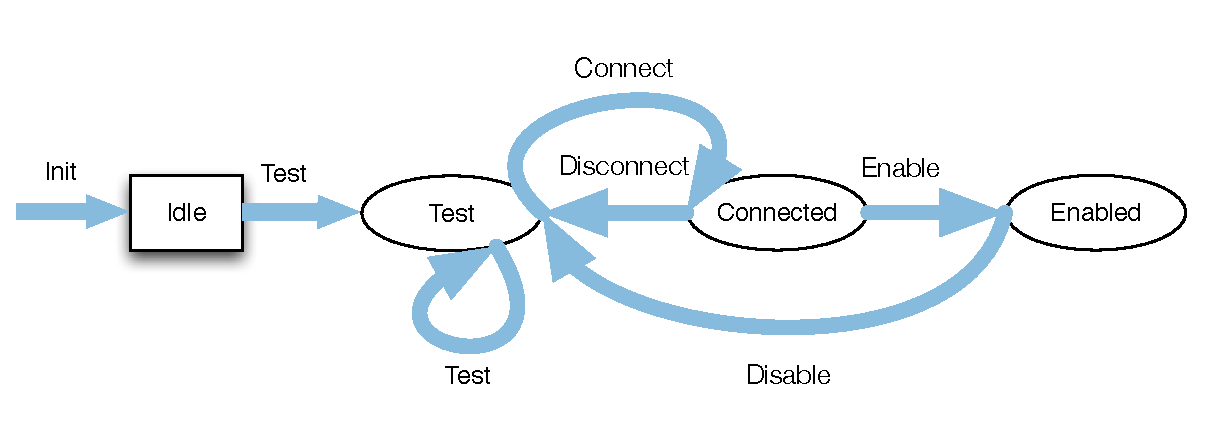
\includegraphics[width=0.6\textwidth]{signpost-tactic}
  \end{center}
  \caption{\signpost tactic lifecycle}
  \label{fig:signpost-tactic}
\end{figure}

In \signpost  we have developed a generic model to encapsulate the testing and
control requirements for connection establishing mechanisms, which we call {\it
  Network Tactic}. Using this model, we aim to automate the setup process for
end-to-end paths.  A \signpost Network Tactic is modelled as a 4 state
automaton.  The state space diagram is presented in
Figure~\ref{fig:signpost-tactic}. A Tactic is initialized in the Idle state. A test
method invocation transfers the tactic to the testing state and runs the
tactic-specific connectivity tests to discover network policy and configuration
requirements.  If testing is successful, the Tactic is able to transfer to the
connect state through an invocation of the connect method. The connect method is
responsible to configure an end-to-end path using the tactic connection
mechanism. Once the end-to-end path is established, the Tactic can progress to the
enabled state and forward traffic over the path.  Finally, the Tactic automaton
provides methods to backtrack from each state and clear stored state. 
% In order
% to avoid packet reordering, \signpost permits the parallel existence of multiple
% connected tactics for a set of devices, but a single path can be enabled at
% any point.

Furthermore, because we require a mechanisms to allow distributed
synchronisation and execution of tactics, we, additionally, define an
architecture to split tactic functionality between the \signpost controller and
client.  The functionality of a \signpost tactic is split logically in two
layers: the Southbound layer, implementing low level tactic operations, and the
Northbound layer, translating the tactic abstraction into low level operations.
The Northbound layer runs on the \signpost controller, while the
Southbound functionality runs on the \signpost clients.  The two layers of the
tactic, communicate over the control channel using a Json-RPC-based 
tactic-specific protocol. 

As an example of this functionality split, we present the Test method of the
\openvpn tactic, an IP tunnelling mechanism using certificate-based
authentication and functioning over TCP or UDP\@. In the test section of the
Southbound layer, the tactic implements two methods: {\emph init} an \openvpn
server with default configuration and {\emph test} client accessibility towards
an \openvpn server on a specific IP and port. The Northbound layer of the tactic
expose a single test method, which instructs participating devices to initiate
an \openvpn server and test connectivity towards the other device. The first
client returning a successful test result becomes the client of the \openvpn
tunnel. If the test times-out for both devices, then the controller initialises
an \openvpn server and instructs the devices to test \openvpn connectivity
towards the controller.

% In the development of the 
% we also consider the way that the
% design can encapsulate the complexity to address the problem of increased
% heterogeneity of the level of connectivity that a Network Tactic provides, we
% include two equally important details in the abstraction. Firstly, each tactic
% can directly modify the forwarding table of the OpenFlow Switch and receive
% feedback from the forwarding plane. In this way we can incorporate in the
% architecture tactics that provide port-based connectivity, as well as network
% layer connectivity. Secondly, because we are interested to allow user
% flexibility on the properties Tactic synthesis in order to enable complex
% combinations of Tactic that can fulfil user policy, we introduce in the design a
% simple mechanism to express meta-data informations on the connection
% requirements of a 


\subsection{Forwarding} \label{signpost-forwarding}

\signpost connectivity is exposed to applications  at the network layer of the
host, providing strong backward compatibility with existing decentralized
applications. A \signpost cloud is abstracted as a local subnet and persistent
local IPs are allocated to each user device. \signpost has a fundamental requirement on
each device, for a network forwarding control mechanism, like the \of protocol,
in order to exercise dynamic network control on each host. The \signpost network
control is responsible to regulate traffic forwarding and detect connectivity
degradation.
% In order to modify the forwarding
% logic of the end-host, we add a requirement for an \of switch running on the
% local system which will be connected to the embedded \of controller of the
% \signpost software. 

The core of the \signpost system exercises minimal control over network traffic
and primarily functions as a multiplexer of control traffic between Tactics.
Non-\signpost traffic is routed as normal by the network stack.  For \signpost
traffic, the \signpost agent delegates network control to the Tactic which is 
responsible to provide connectivity towards a specific remote \signpost host.
Tactics can exercise control either pro-actively or re-actively and,
additionally, they are able to inject and intercept traffic. In
section~\ref{sec:sp-implementation}, we present in detail integration examples
between the \signpost core design and various connection establishing mechanisms
and discuss how network integration is achieved through appropriate control
plane design.  Finally, in order to reduce broadcast traffic on the
\signpost overlay, we integrate in the control plane of the host a simple
ARP proxy which replies with the MAC address {\it fe:ff:ff:ff:ff:ff}\/ to every
ARP request for any \signpost IP addresses. 

\subsection{Connection Manager} \label{signpost-engine}

End-to-end path management in \signpost is encapsulated in the Connection
Manager Subsystem.  The Connection Manager controls path establishment, selects
the optimal path between a pair of devices and ensures connectivity.  Path
selection is modelled as a dynamic optimization problem with security
requirements modelled as constraints and path performance modelled as the
objective function.  Path performance is represented by a positive integer
weight, with higher values reflecting lower performance for the path. The weight
of a path is equal to the sum of the individual weights of the Tactics used to
form the path. Tactic weight, in the current implementation of the system, are
empirically defined through a set of simple rules of thumb. Tactics that include
the Controller in the forwarding path have a higher weight than direct paths.
Similarly, Tactics using connectionless protocols, like UDP, are considered more
efficient than Tactics using connection-oriented protocols, like TCP\@.  Using
these simple rules of thumbs we are able to select the most efficient path, but
more accurate performance characterisation mechanisms can be developed using
active performance measurements. 

Additionally, \signpost defines a simple security model for users to express
security requirements. Security in \signpost has three dimensions:
\textit{encryption}, \textit{authentication} and \textit{anonymity}.  Each
Tactic provides a subset of these three properties, based on the capabilities
provided by the underline connection mechanism. An encrypted Tactic applies
strong cryptography on both directions of the end-to-end path. An authenticated
Tactic uses strong authentication to establish end-to-end paths.  Finally, an
anonymizing Tactic provides end-to-end paths which obfuscate user identity from
eavesdroppers.  Additionally, in order to enable security flexibility, the
\signpost architecture allows {\it Tactic synthesis}. A path is constructed by
forwarding Tactic traffic using the path of another Tactic, creating a layer of
Tactics. For example, an anonymized and encrypted path can be established
through an SSH tunnel running over a TOR circuit between the two devices.
End-users can use security properties to define security policies towards
specific devices. The policy is expressed through a configuration file and users
specify security requirements on a per domain basis. 

\signpost is able to establish multiple end-to-end paths between two devices.
Unfortunately, multipath connectivity is not supported by popular transport
protocols and newer protocols like SCTP and multipath TCP, supporting multipath
connectivity, are not yet available in production systems.  As a result,  in
\signpost we establish and use a single end-to-end path between any pair of
devices.  \signpost path search runs on the \signpost-controller and uses a
simple width-first search algorithm over the complete space of  Tactic
combinations. The search is initiated by the connect method of the Connection
Manager module, with parameters the names of the devices and a list of security
properties. The Manager is responsible to establish an initial end-to-end path and
return successfully. 

The logic of the search algorithm is pretty simple. During a connection request
the system spawns a thread for each Tactic, testing end-to-end connectivity.  If
the test is successful, the Tactic is instructed to connect the two end-points.
If the connection is successful and either there is no other Tactic enabled or
the currently enabled Tactic has a higher performance weight, then the Manager
will progress the state machine of the Tactic to the {\it Enabled}\/ state and
disable any existing enabled Tactics. If the Tactic doesn't fulfil the security
policy, the Manager recursively tests tactic connectivity over the established
path to find Tactic synthesis with sufficient security properties. The Manager
returns a successful result, when the search establishes an end-to-end path
compliant with the security policy.  In addition, the Manager will continue to
search for other lower weight paths between the two devices.  The recursion
terminates if all remaining Tactic combinations have a higher performance weight
or they are synthesized by more that three Tactics. As a result, the Manager can
establish rapidly an end-to-end path between two devices and progressively
optimize path performance, while the devices remain interconnected. 

\subsection{Effectful Naming} \label{signpost-naming}

The majority of Internet-connected devices are essentially anonymous from a
network perspective and assigned transient names (e.g.,~via DHCP). The IPv6
protocol~\cite{RFC1883} addresses a number of such limitations, but the protocol
deployment on the edges of the Internet is slow and, thus, limited. A
fundamental set of requirements for the \signpost architecture is support for stable
device  names and a secure mechanism to resolve these names into
concrete end-to-end paths.  \signpost naming functionality is established
through the DNS protocol~\cite{RFC1034} for two main reasons.  Firstly, DNS is
an effective solution for the naming problem. DNS is an Internet-wide and
accessible service, which is never blocked by the local network. Additionally,
the introduction of the DNSSEC protocol extensions provides a sufficient
mechanism for bi-directional authentication.  On the other hand, the DNS
protocol carries significant information on the user connectivity intentions. 
% Internet hostname function as
% an indirection mechanism providing the ability to decouple the interest of the
% user to connect to a specific service from the real server which will be used. 
The Internet naming service is a delay-tolerant mechanism for applications to
express the interest to connect to a host. DNS domain names represent
fundamentally Internet services, decoupled from the network layer technology,
while the naming format provide a good match to spoken language. 

Domain naming provides good scaling properties, using a hierarchical
architecture. Every domain name consists of a sequence of name tokens organised
in a hierarchical tree structure with a single root, the empty string. Every
node on the tree can be coupled with a number of DNS Resource Records (RR) and
provide a wide range of information for the specific domain name like its
network addresses, possible name aliases and lists with available services. In
order to scale the performance of the naming service across the Internet, the
design of the system allows delegation of service for a specific subtree of the
naming hierarchy to other servers through the NS RR type. 
% As a result, if a host
% knows the IP address of a single DNS server, he can browse the DNS tree and locate
% available information for any DNS domain name. 
In addition, the DNS service
defines a record caching mechanism, to improve lookup performance and service
load. 

% \begin{itemize}
% \item\emph{Ubiquity}. DNS is among the most widely deployed services on the
%      Internet. Effectively every Internet-connected client supports name
%      resolution, and has access to the DNS when connected. 
% \item\emph{Reach}. As such a critical part of the Internet's infrastructure, and
%      unlike TCP, HTTP and similar protocols, DNS tends not to be manipulated by
%      middleboxes other than modified DNS servers
%      themselves~\cite{rfc:3234,handley-mbox}.
% \item\emph{Security}. The DNSSEC security extensions have recently been deployed
%      on the live root servers~\cite{rfc:4033}.  DNSSEC provides origin
%      authentication and integrity protection for DNS records, and (along with
%      SSL) represents one of the two global public key infrastructures.
%    \end{itemize}

% Details of the DNS protocol can be found in RFC 1035~\cite{RFC1035} and its
% many extensions and updates in the RFC repository. Before we discuss Signposts
% in detail, it is necessary to briefly recap key elements of DNS.

% \paragraph{A Brief DNS Recap}
% 
% DNS clients make requests of \emph{resolvers} which in turn issue appropriate
% \emph{queries} concerning the \emph{domain name space} to servers. The domain
% name space is a tree where nodes and leafs correspond to (potentially empty)
% \emph{resource sets} (RRsets) containing one or more \emph{resource records}
% (RRs), where each node has a \emph{label} and its domain name is the sequence of
% labels from the root. A subtree for which administrative responsibility has been
% delegated is referred to as a \emph{zone}. Each query concerns a \emph{target
%   name} and specifies a \emph{query type} and \emph{class} which are used to
% restrict the RRs returned. A \emph{fully-qualified domain name} (FQDN) refers to
% the complete sequence of labels back to the root of the tree; a subset of that
% sequence from a leaf is simply a \emph{domain name}.
% 
% A DNS packet (queries and responses)  contains a standard header and four
% sections: the \emph{question}, containing the name being looked up; the
% \emph{answer}, containing RRs answering the question; the \emph{authority},
% pointing to an authoritative server for the question; and the \emph{additional}
% records, containing any additional information pertaining to the question. Name
% resolution then follows one of two paths. A \emph{recursive resolution} occurs
% when the server does not have the answer and so it acts as a resolver itself,
% pursuing the answer on behalf of the client. In contrast, an \emph{iterative
%   resolution} occurs when the server does not have the answer and responds by
% referring the client to a server ``closer'' to the answer.

\paragraph{Secure Names For All Internet Users}

\begin{figure}
  \centering
    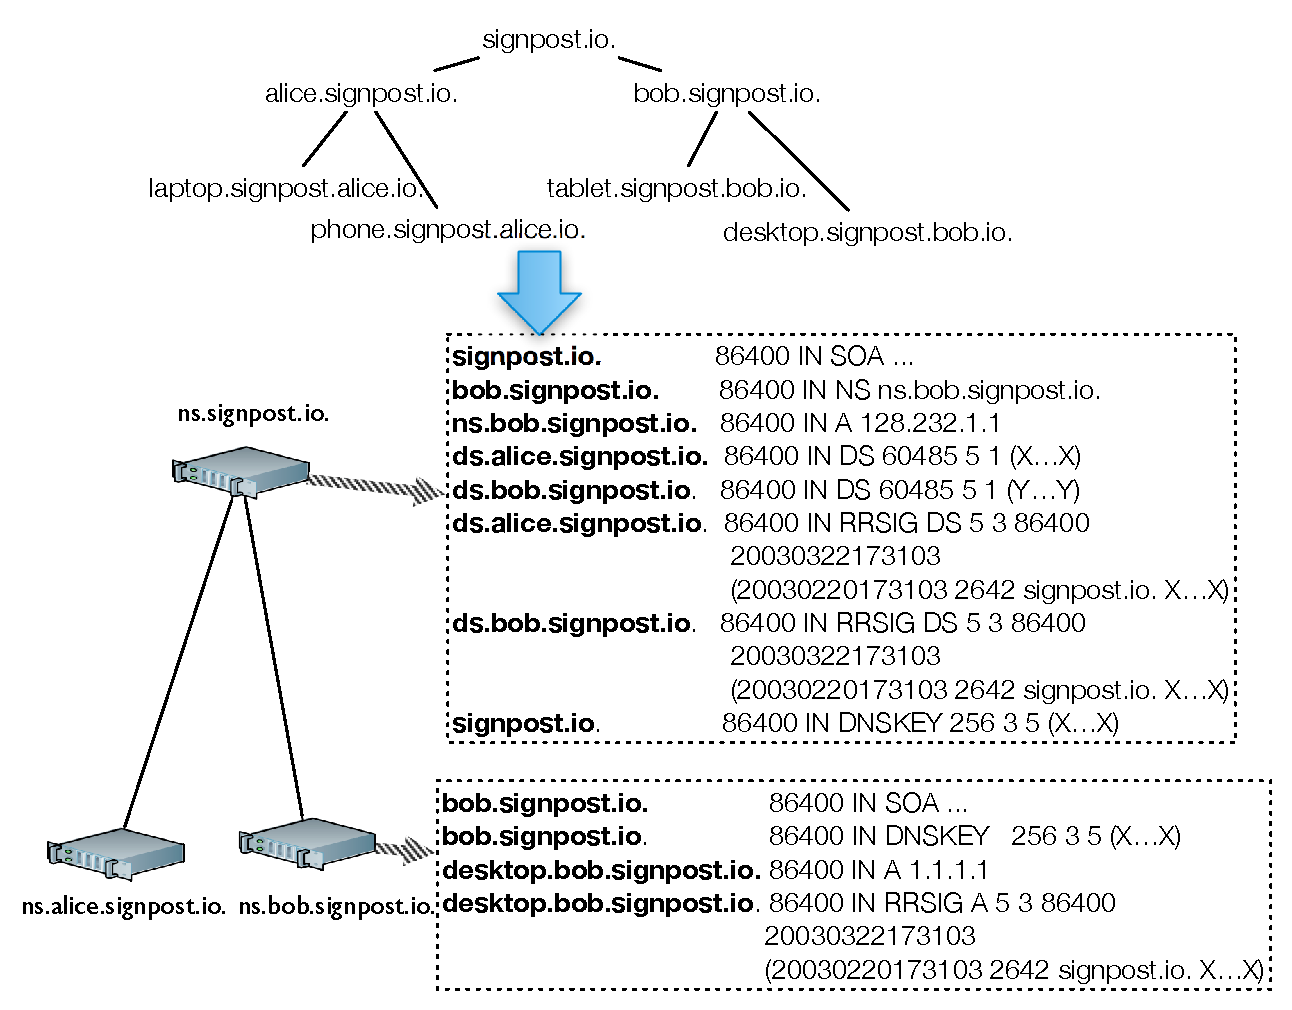
\includegraphics[width=0.8\textwidth]{DNSSEC_hierarchy}
    \caption{DNSSEC key configuration for the io. and bob.io. domains. The io.
      nameserver zone file contains a DS RR with the hash of the bob.io. DNSKEY
      RR and an RRSIG RR signature of the DS RR signed with the DNSKEY of the
      io. domain. bob.io. uses its DNSKEY to sign an A RR for desktop.bob.io.}
  \label{fig:dnssec_hierarchy}
\end{figure}

In the initial definition of the Internet naming service, the protocol provided
very weak security guarantees. In order to enhance the security primitives the
IETF standardised a number of DNS protocol extensions, described as \dnssec.
\dnssec defines three RR types~\cite{RFC4034}, enabling authenticated response
for the protocol. We present the authentication mechanism in
Figure~\ref{fig:dnssec_hierarchy}. In \dnssec, each zone owns at least a
cryptographic key  sign authoritative data using public key cryptography.  The
signature of an RR are transmitted using the RRSIG RR type, while the NSEC RR
type can be used to inform the request of the luck of a respective record type.
The DNSKEY RR type disseminates the public keys of a server to resolvers to
authenticate record signatures and the DS RR type allows a domain to express his
trust to the signing keys of another domain. With respect to
Figure~\ref{fig:dnssec_hierarchy}, the domain \fqsn{bob} signs an A record for
the host \fqsn{desktop.bob} through an RRSIG RR using bobs DNSKEY. The bobs key is
registered in the  io. domain with a DS record containing the hash of bob's key
and signed with the signing key of the io. domain. 
  As as result, the \dnssec
extensions form a chain of trust within the naming service, ensuring the
authenticity of any query response . The resolver requires, as in the X509
certificate architecture, only a list of authenticated anchors configured
out-of-band of the protocol and injected in the authentication chain.

\signpost uses extensively the \dnssec RR types to establish an authenticated
control channel between the devices of the user. For each user of the \signpost
system, we require control delegation of a domain to the \signpost controller
and registration of the domain signing key to the \dnssec chain of trust. Each
device has a domain name under the domain  of the user. With respect to
Figure~\ref{fig:signpost-arch}, Bob is granted control of the domain \fqsn{bob}
where she registers her laptop under the domain name \fqsn{laptop.bob}. As a
result, each \signpost user has a globally accessible authenticated public
identity for each device via a public-private key-pair. Using this key-pair, a
user can sign and authenticate messages, bootstrap public key cryptography
mechanisms and run key-exchange mechanisms such as
Diffie-Merkle-Hellman~\cite{RFC2631} and derive new shared private keys between
any two devices over unsecure channels.

The base \dnssec RR types  provide a mechanism to authenticate responses from a
nameserver to a DNS resolvers. In terms of the \signpost architecture, we are
interested additionally to authenticate DNS requests. Authenticated requests
enable the server to present a different view over the resource mappings,
depending on the querying entity.  \footnote{{\em ``DNS servers can play games.
    As long as they appear to deliver a syntactically correct response to every
    query, they can fiddle the semantics.''---\,RFC3234~\cite{RFC3234}}}
\signpost uses the SIG(0) RR type, defined in~\cite{RFC2931}, to sign DNS
requests using the key of the device.  
% The record was introduced in order to allow authorized
% clients to update RR records on an authoritative server, while it permits a
% client also to point to the signing entity, in order to fit the authentication
% within the \dnssec key structure. 

% Using DNSSEC here instead of SSL has several important advantages. Firstly,
% DNSSEC has maintained the integrity of its trust chain better than SSL (which
% has a large set of root certificate providers), and has explicit support for
% incomplete trust chains via look aside validation~\cite{RFC5074}.  Secondly,
% DNSSEC has few network dependencies and exploits all of the distributed benefits
% of DNS, such as caching, proxy lookups, and a low-latency protocol.  Lastly, a
% domain also has a single, well-defined owner if registered under a top-level
% domain, whereas URL-based identity schemes such as
% OpenID~\cite{Recordon:2006:OPU:1179529.1179532} depend on trusting the
% underlying owner of the domain for that URL.\todo{will we discuss icann
%   implications of so many new internet names later on?}

%% \subsection{Centralised Named Routing}
%% \label{s:topo1}

\paragraph{Fitting \dnssec in \signpost} 

\signpost evolves the default DNS processing logic on the client and the
controller of the architecture. On the controller we develop a programmable DNS
server functioning as the authoritative server for the user domain. The server,
beyond serving domain records and signing responses on-the-fly, can additionaly
verify SIG(0) signed queries and translate them into Connection Manager
requests. A request for an A RR for domain name \fqsn{laptop.alice}, signed with
a SIG(0) record with a key from host \fqsn{desktop.alice}, will be translated
into a connection request between Alice's laptop and desktop devices.  
% In order to enforce liveness of \signpost
% RR records in the Internet, we set a zero TTL value on all RR records, thus
% disabling any DNS caching.

In the client side of the \signpost architecture, we use a local \signpost-aware
DNS resolver. DNS queries for non-\signpost hosts triger a recursive search of
the DNS name tree, in order retrieve required RRs.  For \signpost host request,
the resolver sings the query with a SIG(0) record using the private key of the
device. 

Using the DNS protocol we are also able to provide offline functionality for two
devices disconnected from the \signpost Controller, but connected to the same
network, by using DNS-based service discovery~(DNS-SD)~\cite{RFC6763}.  DNS-SD
is an RR organisation specification which wnables service advertisement and browsing
over the Multicast-DNS~\cite{RFC6762} service and effectively providing an efficient
local service discovery mechanism. The combination of DNS-SD and multicast-DNS
is currently a popular service discovery mechanism in local networks,
supported by most operating systems.  The \signpost system 
advertises , using the DNS-SD mechanism, a \signpost service record with name
\_sp.\_tcp.local in the local network along with an RRSIG RR and the DNSKEY RR of the device, signed with the
private key of the domain. As a result, a \signpost client can
verify a destination \signpost service and establish a control channel. 
% This way each device in the local network can listen for the service service
% name and once a new node appears, it can verify the validity of the service.
During the offline  mode, the query receiver will function as a
\signpost Controller, responsible to server RR request for its domain name only. 

% \paragraph{Putting It Into Practice} Having established a secure identity, we
% require the means to signal a communication channel between any pair of a user's
% devices, no matter the middleboxes and other impediments between them. 
% %In this section we discuss how we adopt the increasingly widely deployed
% %DNSSEC~\cite{Friedlander:2007:DPT:1247001.1247004} for device naming, via a
% %Signpost DNS server ``in the cloud'', and a guaranteed route-of-last-resort
% %tunnel from every device to this server.
% 
% %along with a guaranteed \emph{route-of-last-resort} available through Signposts
% %that provides the latter. Where there are many possible such routes, the
% %``best'' should be chosen, ``best'' being, as ever, application dependent. We
% %discuss construction of higher bandwidth, lower latency routess that make
% %better use of localised resources later~(\S\ref{s:topo2}).
% 
% To make this concrete, consider a simple scenario. Alice has a \signpost server
% running in a globally visible location in the public cloud. This serves her
% public key and zone, \fqsn{alice}, with DNSSEC providing a chain of signed
% attestations back to the DNS root that the record has not been tampered with en
% route. Alice has two network-connected devices, her phone and home desktop.  As
% is typical, her phone's 3G network connection is gatewayed by her mobile
% provider and her home computer is behind a NAT. Thus
% none of her devices are readily reachable directly by each other, or by others
% via the Internet.
% 
% Connecting these two devices currently requires Alice to manually configure a
% tunnel at her NAT box, or to run VPN software on her phone. No automatic
% signalling mechanism exists to setup these connections on demand, nor even to
% address the devices by a global name. With \signpost, Alice binds the concrete
% names \spsn{phone} and \spsn{home} to her devices, and runs a publicly visible
% server hosted in a cloud to coordinate their name resolution.
% 
% Establishing a connection between \spsn{phone} and \spsn{home} via the \signpost
% is then relatively straightforward. One client, say \spsn{home}, initiates the
% process by attempting a DNS resolution of \fqsn{phone.alice}. Normal DNS
% mechanisms cause this query to reach Alice's \signpost, which has been delegated
% the zone \fqsn{alice}. It resolves the name \spsn{phone}, causing various
% \emph{tactics} (\S\ref{s:topo2}) to be executed, the result of which is that a
% VPN is established between Alice's phone and computer, and a valid IP address
% endpoint returned in the DNS query.
% 
% \todo{Somewhere in this section we need to mention Signpost Clients and Signpost
%   Servers -- and the difference between `client' devices. Otherwise the
%   distinction gets confusing later in the report.}

\subsection{Security and Key Management} \label{signpost-security}

\signpost develops a public key distribution mechanism for each user device
integrated with the \dnssec protocol and, thus, enables seamless inter-device
authentication and strong security bootstrapping.  We use a three layer key
hierarchy to enable dynamic trust control and revocation over device keys.
\signpost key hierarchy extends the key hierarchy defined in the \dnssec
protocol. A \signpost cloud has at least two RR signing keys: A {\it Zone
  Signing Key (ZSK)} and a {\it Device Signing Key(DSK)}. ZSK is used to sign
the DSK, while the hash of the ZSK is stored as a DS RR in the top-level name
servers. DSK is used by the controller to sign device keys, as well as,
authoritative RR. The separation of the authentication mechanism between two
keys allows a user to maintain a persistent anchor in the \dnssec key chain and,
in parallel, be able to revoke trust for a key of the domain without having to
propagate the change to a server beyond the user control.  Each registered
\signpost device must construct a Device Key and add it securely in the zone
file of the Controller, in order to be able to join the user cloud. The device
public key is added in the zone file of the Controller through a DNSKEY record
and the controller will construct an RRSIG RR for the key using the DSK in order
to express its trust on the key and effectively allowing other devices to
verify the identity of a device. Any device with an anchor in the global \dnssec
key infrastructure can verify any \signpost signed request, by following the
key chain in the \dnssec tree.

\section{Evaluation}\label{sec:signpost-evaluation}

In this section we analyse the performance of the \signpost system and present
our experience from using a number of distributed Personal Cloud applications

thas replace popular centralised Personal Clouds. Specifically, we present the
implementation details of a strawman implementation of \signpost
(Section~\ref{sec:sp-implementation}), measure the performance of the \signpost
tactics over the Internet~(Section~\ref{sec:sp-tactic-eval}) and present a small
scale study of the functionality of current application over the \signpost
system. 

\subsection{\signpost implementation} \label{sec:sp-implementation}

\signpost is implemented predominantly in Ocaml and uses existing protocol
libraries to integrate DNS and \of protocol support to the core daemon of the
system.  More specifically, we employ the ocaml-dns library for DNS server and
client functionality, the cyptokit library for cryptographic key manipulation
and the ocaml-openflow library for \of controller implementation. \signpost also
uses a portion of C code to implement binding with the OS routing stack. Our
strawman implementation is fully functional under Linux and Android, using the
\ovs switch implementation, and MacOSX, using the userspace switch
implementation provided by the ocaml-openflow library.

The \signpost Tactic model is able to encapsulate the testing and configuration
requirements for the connection establishing mechanisms: 

\begin{itemize}

  \item \emph{Direct}: The tactic establishes communications paths between
    devices tests and evaluates the ability for two device to connect directly
    over the network without any tunnelling mechanism. After a name lookup, the
    tactic tests if direct bi-directional connectivity is possible between the
    two devices for a set of popular ports (e.g. TCP and UDP connectivity
    through the ports 53, 80, 443 and 8080). If the tests are successful, the
    tactic insert a couple of \of rule on both devices to translate \signpost
    device addresses to the network addresses which have been successfully
    tested. 

  \item \emph{\openvpn}: The \openvpn tactic establishes connectivity using the
    \openvpn tunnelling mechanism. During testing, the tactic tests connectivity
    over UDP to port 1194 between the devices, as well as, towards the
    controller. If the test was successful, \signpost devices  use the \signpost
    key infrastructure to generate public keys and bootstrap the \openvpn
    authentication mechanism.  Because of some limitation on the certificate
    chain evaluation of OpenSSL, during a connection the Tactic generates
    transient private keys, signed by the user private key, while the tactic
    will inject in the trusted certificate keychain a key certificate of the
    destination device signed by its private key.  The tactic configure the
    \openvpn software to expose connectivity over an Ethernet TAP
    device~\cite{tuntap}, which is added under the control of the \of switch.
    Because the \openvpn software contains a small ARP cache, we assign a unique
    IP in the 10.0.0.0/8 subnet to each TAP device and broadcast appropriate ARP
    notification packets.  The tactic, similarly as in the Direct tactic,
    inserts \of rules on all participating devices to forward packet over the
    \openvpn tunnel, while translating appropriately the source and destination
    addresses. 
%     rules establish full bi-directional connectivity.  
%     \todo{Mention OpenVPN ARP cache}

  \item \emph{SSH}:  The tactic provides inter-device connectivity over the SSH
    protocol. For this tactic we configure and run an SSH daemon on every
    \signpost device on port 10000, permitting only key-based tunnelling
    connectivity.  Tactic testing evaluates the ability to establish a TCP
    connection between the device or through the Controller.  Connectivity
    enforce strong user authentication by using the key-based authentication of
    the SSH protocol. \signpost device servers append device public keys in the
    authorized\_key file in an ad-hoc manner and clients use the private key of
    the device upon connection on their SSH client.  The SSH tactic associates
    the SSH tunnel with a local TAP Ethernet interface on each device and the
    tactic controller insert appropriate \of rules to forward traffic towards
    the relevant TAP interface.

  \item \emph{Privoxy}: This tactic enables HTTP request anonymization using the
    Privoxy~\cite{privoxy} HTTP proxy. The tactic configures a privoxy HTTP
    proxy server on each device, configured with a strict policy to anonymize
    privacy leaking HTTP headers.  In order to establish connectivity, the
    tactic handles TCP flows in a proactive manner.  For each SYN packet, the
    tactic install bi-directional flows, forwarding data from the application to
    the local listening port of the Privoxy daemon.


\begin{figure}
  \begin{center}
	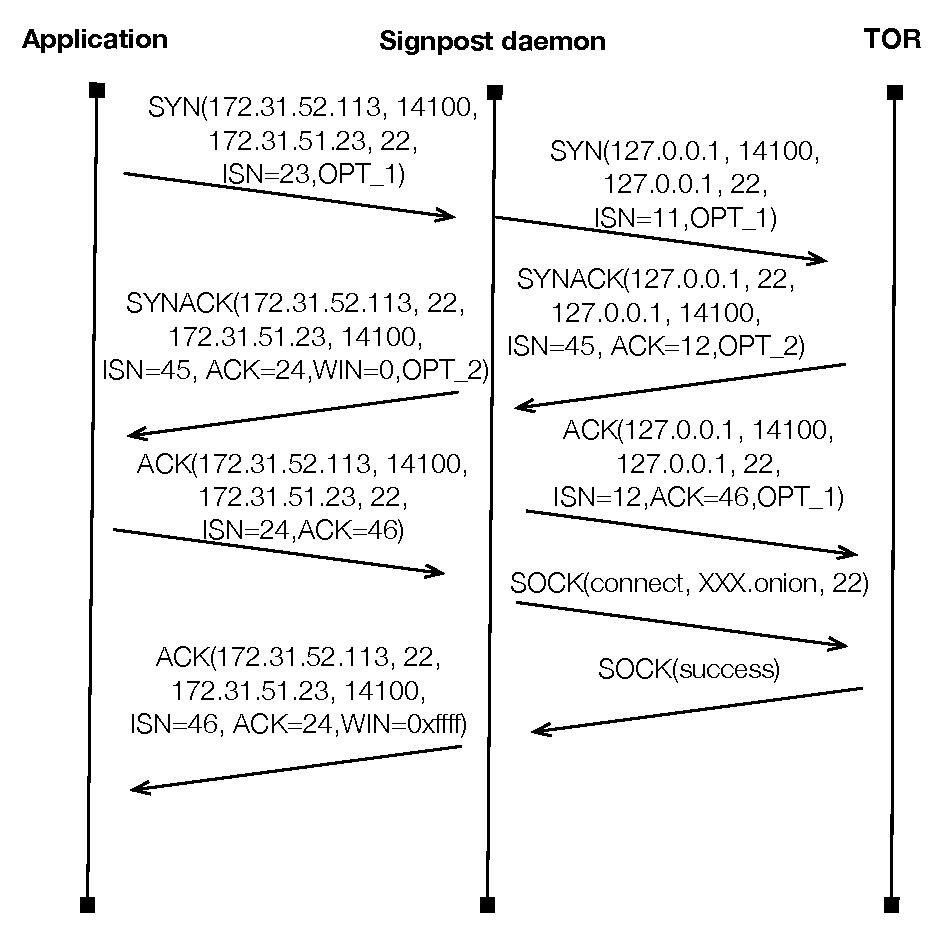
\includegraphics[width=0.7\textwidth]{tor-example}
  \end{center}
  \caption[TOR tactic implementation in \signpost]{TOR tactic implementation in
    \signpost. The local \signpost daemon translates new TCP connection requests
    towards the destination device to appropriate SOCK request to the SOCK proxy
    of the software.}
  \label{fig:signpost:tor-example}
\end{figure}
  
  \item \emph{TOR}: The TOR tactic enables connectivity between devices over the
    Anonymized network of Tor~\cite{dingledine2006}. The tactic configures a TOR
    client on each device, providing a SOCKS proxy which forwards TCP traffic
    through the TOR network.  Additionally, the tactic takes advantage of the
    hidden service functionality of the TOR system, which allow TOR nodes to run
    anonymized services. In order to achieve this, TOR generates for each host
    an anonymized domain name under the .onion domain and employs the embedded
    name lookup capability of the SOCKS protocol. The TOR testing method is 
    primarily responsible to initialize the TOR daemon, propagate the
    domain name of the device to the Controller and test the effectiveness of
    the tactic in the network environment.  Testing and setting up of TCP flows
    using the TOR tactic follows a simple \of-based mechanism. The TOR
    initially insert an \of rule to forward all packets towards the
    \signpost IP of the remote host to the controller. Upon a SYN packet
    transmission from an application to the remote \signpost host, the tactic
    will initiate a TCP connection with the local SOCKS proxy with a request to
    establish a path between the two devices. In parallel, once the TCP
    connection is established with the local SOCKS proxy, the tactic will
    respond to the initial SYN request with a SYNACK packet with appropriately
    modified sequence and ACK numbers to accommodate the additional bytes of the
    SOCK protocol interactions with the proxy and advertise a zero
    window, in order to suppress any further data transmission from the
    application.  Once a SOCKS response is returned by the TOR proxy, the tactic
    will either respond to the initial TCP flow with an ACK with a non-zero
    window and insert appropriate \of rules to permit connectivity between the
    two device over the SOCKS tunnel, or the client will inject a TCP RST if the
    SOCKS response was unsuccessful. A graphical representation of the TOR
    tactic is presented in Figure~\ref{fig:signpost:tor-example}. 
      In order to replicate a similar abstraction
    for UDP and ICMP traffic, we additionally setup a VTUN tunnel over a TCP
    connection, thus enabling IP-level connectivity. Nonetheless, we avoid using
    the tunnel for TCP connections, to reduce capacity loss by the additional
    headers of the tunneling mechanism. 

  \item \emph{DNS-SD}: The DNS-SD tactic enables service advertisement between
    \signpost devices. DNS-SD~\cite{RFC6763} is a common OS service enabling
    hosts to advertise services in the local network.  The main motivation for
    this tactic is to aid existing decentralised Personal Cloud applications,
    which depend on the DNS-SD functionality, to discover the service
    capabilities of connected \signpost devices. The Tactic connect method
    primarily intercept DNS-SD packets from the local stack of the device and
    propagates them over the control channel to the other devices of the user.
    \signpost device must inject equivalent DNS-SD multicast packets through the
    \of protocol to the network loopback device and effectively to the local
    DNS-SD daemon.


\begin{figure}
  \begin{center}
	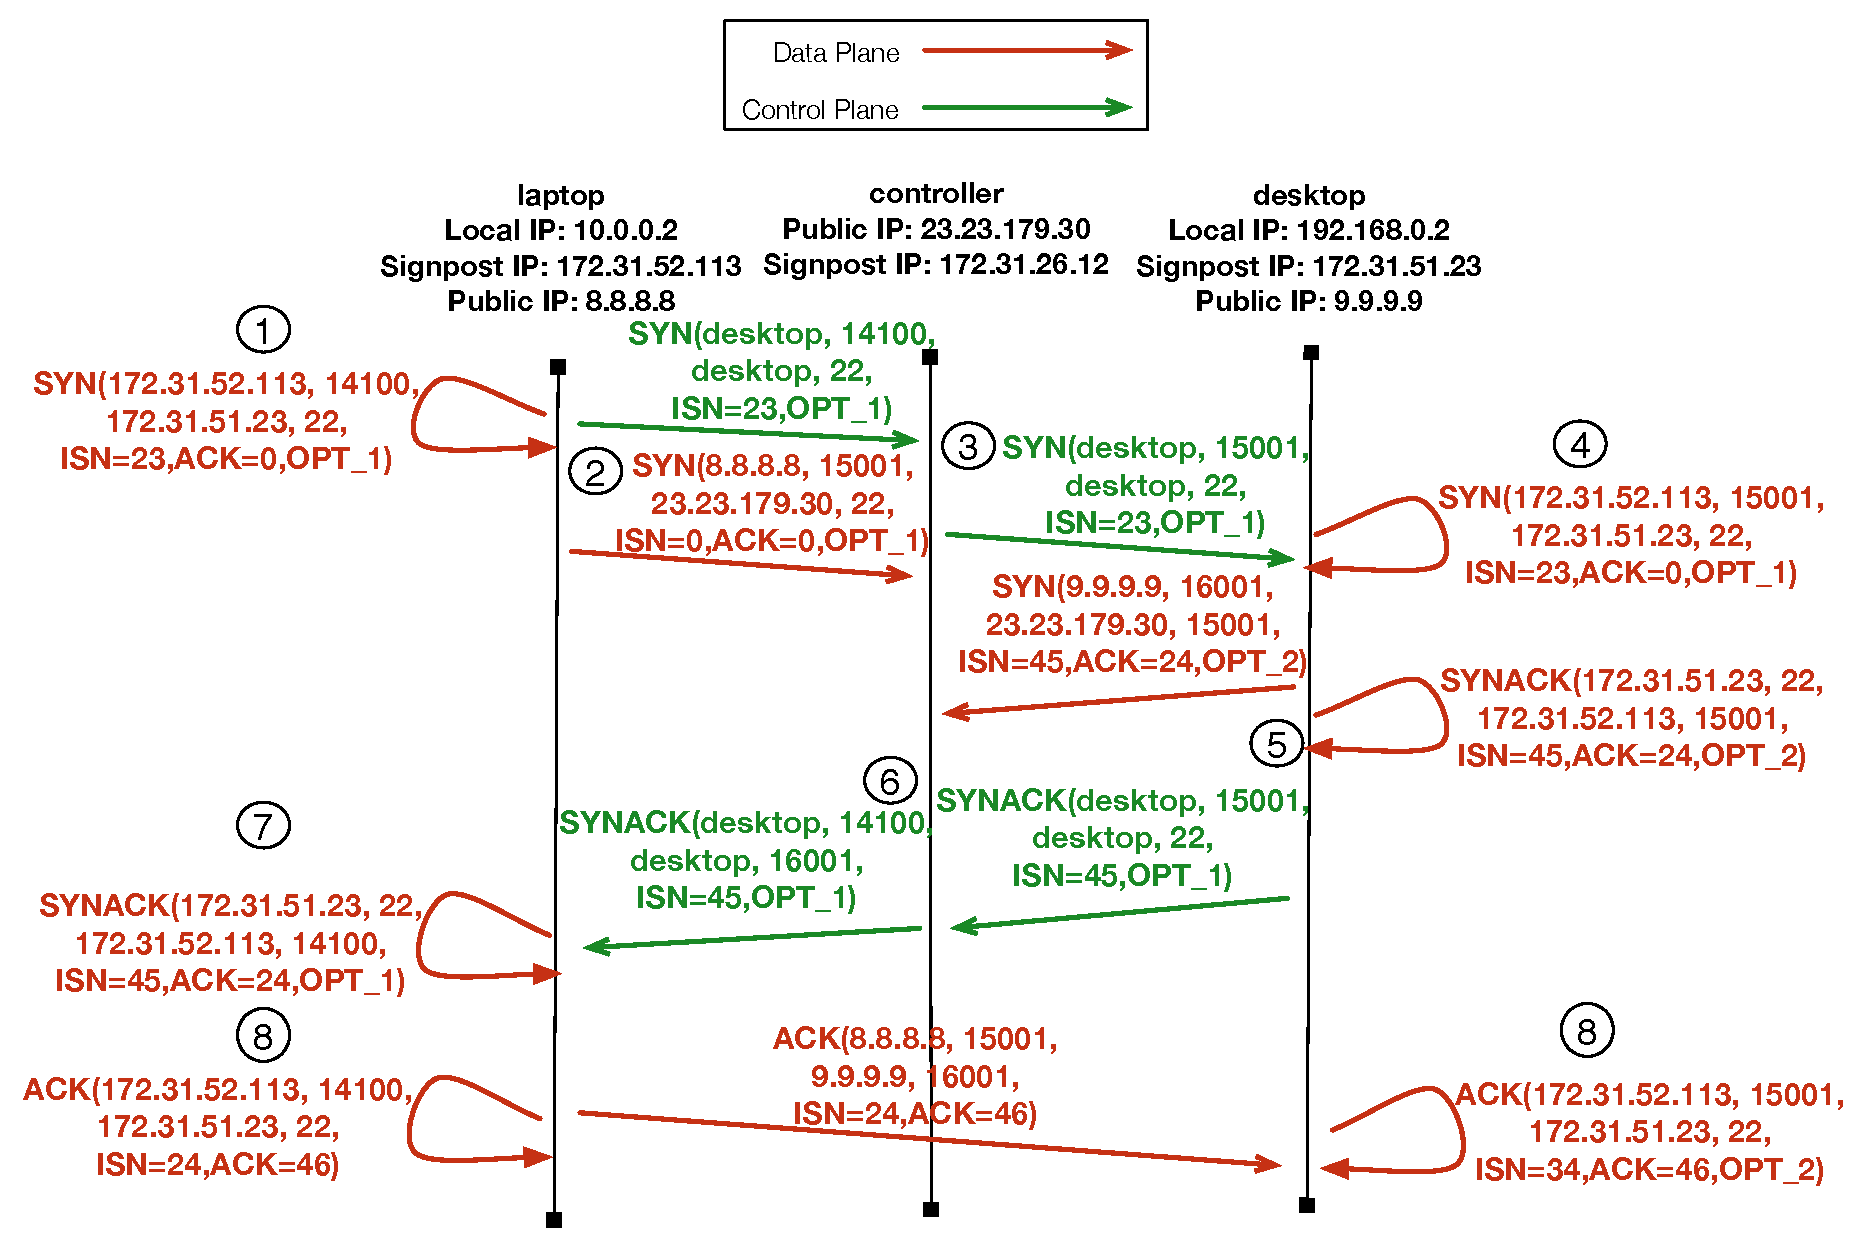
\includegraphics[width=0.9\textwidth]{nat-punch-example}
  \end{center}
  \caption[NAT punch tactic implementation in \signpost]{NAT punch Tactic
    implementation in \signpost. The device local \signpost daemon injects
    crafted packets to create appropriate state in the local network NAT, while
    the controller enables the Tactic to detect the incurred NAT port mapping
    for both hosts of the path.}
  \label{fig:signpost:nat-panch-example}
\end{figure}
  
  \item \emph{NAT-punch}: This tactic implements a packet injection technique which
    allows TCP and UDP flows to bypass NAT boxes. The functionality of this
    tactic is limited and functions only with of Full-cone NAT,
    Address-restricted NAT and Port-restricted NAT, while it is not functional
    with stateful NAT proxies.  The NAT-punching tactic uses the Controller to
    infer the port mappings configuration of the NATbox. We present a schematic
    of the mechanism for a TCP connection in
    Figure~\ref{fig:signpost:nat-panch-example}. Specifically, for new TCP
    connections, the daemon intercepts the SYN packet~(Step~\ding{192}), and
    propagates the important TCP header parameters~(Port number, initial
    sequence number and TCP options) over the control channel to the remote
    device and in parallel send a SYN packet from the device to the Controller
    in order to infer the port mapping applied by the network
    NAT~(Step~\ding{193}). The controller  will extract the source port mapping
    applied by the NAT and forward it, along with the TCP initial sequence
    number, to the destination device, upon the receipt of the SYN packet from
    the flow initiating device~(Step~\ding{194}).  Once the destination device
    receives the control message from the controller, it will generate a SYN
    packet, using the header fields of the initial SYN packet, and send it both
    to the listening service and the \signpost Controller~(Step~\ding{195}). In
    the destination device, the \signpost daemon intercepts the SYNACK response
    of the listening service and propagate the TCP header fields over the
    control channel to the connection initiating device~(Step~\ding{196}).  Once
    the exact port-mapping is inferred by the Controller, the information is
    propagate to the initiating device~(Step~\ding{197}), which will inject a
    SYNACK packet to the local stack to progress the
    TCP-handshake~(Step~\ding{198}). Finally, the two device insert appropriate
    entries in the \of flow table to translate incoming and outgoing traffic of
    the flow~(Step~\ding{199}).

    For UDP traffic, the tactic controller will intercept the initial UDP packet
    of the flow and propagate over the control channel to the remote device, as
    well as, transmit an similar packet to the Controller in order to generate
    appropriate state in the intermediate NATboxes. The remote device will also
    send a similar UDP packet to the Controller Once the controller has received
    both UDP packets, it will notify both devices to insert appropriate flow
    rules to transform IP address and port numbers of the flow and resume UDP
    traffic transmission. 
    

\end{itemize}

\subsection{Tunnel Evaluation} \label{sec:sp-tactic-eval}
\begin{figure}
  \begin{center}
	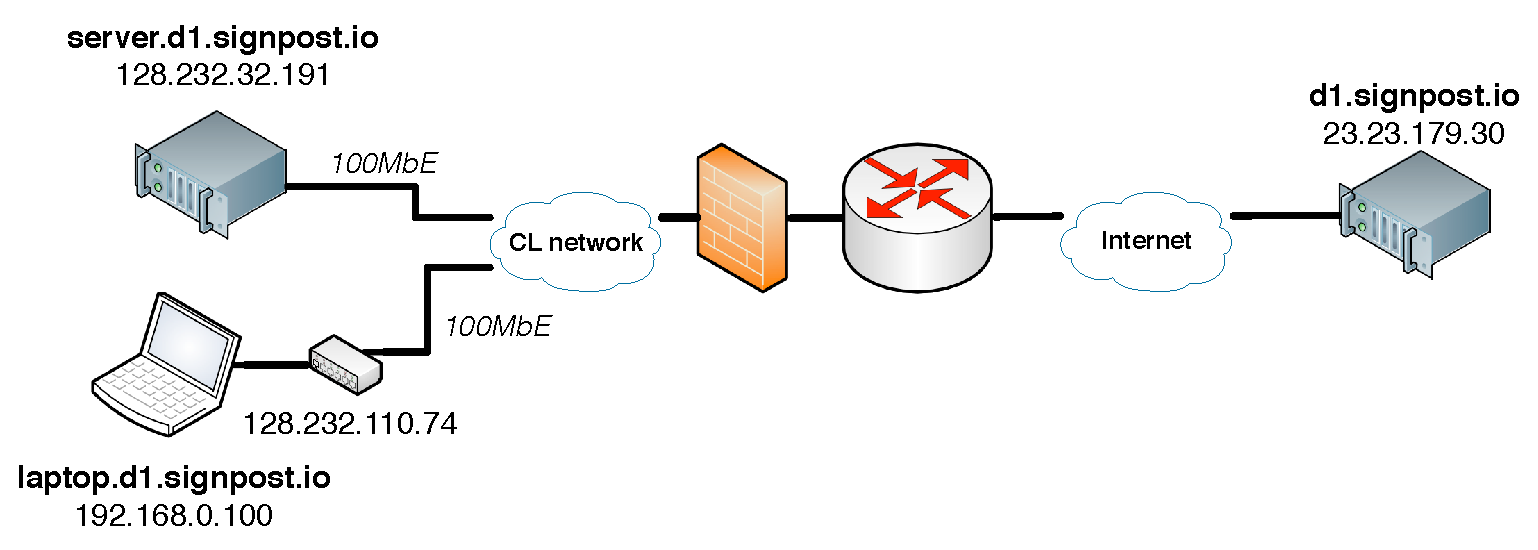
\includegraphics[width=0.7\textwidth]{Chapter3/Chapter3Figs/measurement_topology}
  \end{center}
  \caption[TOR tactic implementation in \signpost]{\signpost tunnel evaluation
    topology. \textit{server} and \textit{laptop} hosts are connect in the same
  network but on different subnets with a firewall enforcing a network security
  between the two devices. The \signpost \textit{controller} is hosted on an
  Amazon ec2 micro instance. }
  \label{fig:signpost:measurement_topology}
\end{figure}
 
\begin{table*}
\centering
\footnotesize
\begin{tabular}{|l|c|c|c|c|c|c| }
  \hline
  \multirow{2}{*}{Tactic name} & \multicolumn{3}{|c|}{Direct connectivity} &
  \multicolumn{3}{|c|}{cloud-based connectivity} \\
\cline{2-7}
& setup~(sec) & throughput~(kbps) & RTT~(msec) & setup~(sec) &
throughput~(kbps) & RTT~(msec) \\
\hline
Direct       & 1    & 94.1 & 1.5  & -   & -     & -   \\
\openvpn      & 13.3 & 66.0 & 1.23 & 20  & 1.9   & 172.0 \\
SSH          & 6.8  & 86.5 & 2.73 & 8.8 & 1.7   & 829.0 \\
TOR          & 60.2 &  2.4 & 912.0   & -   & -     & -   \\
NAT-punch    & 1.2  & 94.1 & 1.5  & -   & -     & -   \\

% iperf -c quorum101.cl.cam.ac.uk  -i 1 -F /dev/urandom -t 60
% fping 172.31.28.49 -e -b 1400 -c 6000 -p 1 -D -s -e -q
\hline
\end{tabular}

\label{tbl:signpost:tactic_perf}
\caption[\signpost tactic evaluation]{\signpost tactic evaluation in terms of
  latency to setup a path, throughput and RTT time. }
\end{table*}

In order to evaluate the performance of our strawman implementation, we conduct
a series of measurements to quantify the impact of the architecture to network
functionality, as well as, the performance of each Tactic.  Our testbed consists
of three hosts, two clients and a cloud controller. The two \signpost
clients~(laptop.d1.signpo.st, server.d1.signpo.st)
are connected to the production network of the Computer Laboratory on different
subnets of the network. The network enforces a security policy both between the
devices,as well as, towards the Internet through a stateful firewall.
Additionally, one of the hosts is connected to the network through a NATed 
home router. The \signpost controller of our experiment runs on an
Amazon EC2 micro instance. The topology of the measurement is depicted in
Figre~\ref{fig:signpost:measurement_topology}. Using \signpost, we establish all possible end-to-end
tactics~\footnote{We exclude the privoxy and DNS-SD tactics, as they don't
  provide end-to-end connectivity, but focus more on providing additional
  functionality to a path} and measure a series of important network performance
parameters.  More specifically, in each experiment we initialize the \signpost
daemon on each device, and establish connectivity using a specific Tactic. For
each established path we measure the latency to setup the path after a name
resolution of the respective host, the throughput of the path, using an Iperf
TCP measurement probe, and the average RTT of the path, using an Iperf UDP
measure probe  of 1~Mbps. We contact our measurement ten times for each possible
configuration and present the median value of the measurements in
Table~\ref{tbl:signpost:tactic_perf}. 

From the result of our experiment we note the difference in capacity and latency
when a path is setted up through the \signpost controller. Edge network
connectivity provides two to three orders of magnitude higher performance than
cloud-aided paths. In addition, we highlight the trade-off between security and
performance between Tactics. For example, although the TOR network provides
strong anonymization functionalities, its performance and latency are inadequate
for a significant portion of modern network applications. The performance
degradation is primarily due to the onion routing scheme used to obfuscate the
destination of a network packet, as well as, due to the sharing nature of the
system.  Nonetheless, the performance and security trade-offs are exposed and
controlled by the end-user through the \signpost control abstraction.
Furthermore, based on the measurement of the path setup latency, we conclude
that the \signpost control plane logic has minimal impact on the host network
functionality. Bootstraping an end-to-end path through \signpost incurs
noteworthy setup latencies for new device paths but the DNS naming service is
designed to handle such latencies~\footnote{Linux has a default timeout of 5
  seconds and 2 retries before timing out a name resolution, providing a budget
  of 10 seconds to a \signpost Tactic to provide a
  response~\url{http://linux.die.net/include/resolv.h}}. Only the TOR tactic
incurs significant latency to setup an end-to-end circuit over the onion
overlay. At the moment our implementation exposes this latency to the user
application, in order to avoid stale TCP connections. This latency can be easily
hidden by the application if a more optimistic flow setup is implemented (e.g.
Assume that an end-to-end connection will be setup between the two devices and
block application by advertising early a zero length window through the SYNACK
packet).  Finally, using the aforementioned topology we also measured the
performance of Tactics synthesis.  From our experiment we report that the
throughput and RTT of such paths is equal to the minimum value between the Tactics
forming the network path, while the setup latency is equal to the sum of
the individual Tactics. 

\subsection{Application compatibility}

In order to evaluate the effectiveness of the \signpost system, we tested our
strawman implementation compatibility with a number of popular applications
providing resource and information sharing.

\paragraph{File Sharing}

In order to evaluate the functionality of file sharing applications over
\signpost we tested three popular data sharing applications: NFS~\cite{RFC5661}, 
git-annex~\cite{git-annex} over rsync and file transfers over the SSH protocol.
We report that all mechanisms function as expected, with noticeable performance
differences proportional to the throughput provided by each Tactic. In our
initial experimentation we had to modify mildly our flow management logic, as
the SSH protocol tends to modify the IP header ToS bits during the transmission
of a flow and requires a wildcarded flow definition.  

\paragraph{Resource sharing}

Using the topology in Figure~\ref{fig:signpost:measurement_topology}, we setup
and test the system support for resource sharing using our strawman
implementation. More specifically, we test support for CUPS remote printing,
DAAP media sharing using the UPnP resource advertisement, VNC remote desktop and
SSH remote access and conclude that our \signpost architecture support the
application functionality.  

\section{Summary} \label{sec:signpost-conclusion}

This chapter focused on the problem of Internet-scale inter-device connectivity.
Our work is motivated by the end-user requirement for resource and information
sharing services between the increasing number of personal devices, a generic
abstraction which we term Personal Cloud. We elaborate on the available
mechanisms providing such functionality and highlight the trade-offs among the
available solutions. We argue that an evolve control plane for end-user devices
can provide a sufficient and secure framework to enable Personal Cloud
functionality, and present \signpost, an evolved control plane for end-user
devices.  \signpost provides network-level secure and user-managed device
interconnection by automating the configuration task of available network
connectivity mechanisms, providing sufficient, secure and backwards-compatible
network functionality to existing distributed Personal Cloud applications. 

\signpost evolves the control plane of the user devices in two aspects. Firstly,
the device control plane is integrated with \textit{Network Tactics}; mechanisms
enabling ad-hoc end-to-end connectivity, like tunneling software and NAT
punching techniques. The architectures develops a generic model coupled with a
secure Internet-wide control channel which provides the ability to orchestrate
the testing and configuration of Tactics between devices.  In addition, the rich
security properties provided by existing network Tactics, allow the system to
expose a security control abstraction, enabling users to define the trade-off
between performance and security when they interconnect their devices.
Secondly, the architecture integrates the control plane logic with the network
naming service. As a result, \signpost provides Internet-wide persistent device
names, while \dnssec naming extensions allow \signpost to construct a secure and
globally accessible key distribution mechanism.

We evaluate our strawman \signpost implementation in terms of its ability to
integrate existing network connectivity mechanisms, its impact in user perceived
performance and its ability to replicate existing Personal Cloud use cases. We
provide evidence on the generality of the \signpost Tactic model by presenting
its integration with a number of connectivity establishing mechanisms, namely
\openvpn, TOR, SSH, NAT punching and DNS-SD.  Additionally, we measure the
performance of inrwgrated Tactics in a typical deployment scenario and verify
the backward compatibility of the system with a number of popular decentralised
applications. In the next chapter, we conclude the results of our research and
discuss future direction of the research.  

% \begin{itemize}
%   \item This is an elementary approach for Personal Cloud computing. 
%   \item A number of issues remain unandressed but can easily fit in the
%         \signpost architecture
%   \item extending the policy mechanism, we can integrate in a Personal cloud
%         devices from other users. Need though to develop a more refined policy
%         that will enable the user to control access from devce outside of its
%         personal to a subset of the available services. 
%   \item Tighter DNS integration of the control protocol.
%   \item 
% \end{itemize}

